\renewcommand\chapterillustration{./abertura-ladrilhos}%Photo by Hoach Le Dinh on Unsplash, https://unsplash.com/photos/c8TWWQ5ZnUw?utm_source=unsplash&utm_medium=referral&utm_content=creditCopyText 
\def\chapterwhat{O ladrilhamento de uma superíficie plana é uma cobertura do plano onde formas (polígonos) são repetidos sem sobreposição ou buracos. Os poligonos utilizados  podem ser  regulares ou não.  Apesar do número de possibilidades de realizar um ladrilhamento parecer infinita, é possivel comprovar que ao utilizar apenas  polígonos regulares existe apenas 11 possibilidades. Contudo pode-se aprofundar o estudo e investigar a utilização de polígonos irregulares}

\def\chapterbecause{O ladrilhamento de uma superíficie plana é uma cobertura do plano onde formas (polígonos) são repetidos sem sobreposição ou buracos. Os poligonos utilizados  podem ser  regulares ou não.  Apesar do número de possibilidades de realizar um ladrilhamento parecer infinita, é possivel comprovar que ao utilizar apenas  polígonos regulares existe apenas 11 possibilidades. Contudo pode-se aprofundar o estudo e investigar a utilização de polígonos irregulares} 
\chapter{Ladrilhamento}
\label{ladri-chap}

\mbox{}\thispagestyle{empty}\clearpage

\thispagestyle{empty}

\begin{center}
Projeto: LIVRO ABERTO DE MATEMÁTICA

\noindent \begin{tabular}{lcccr}

\includegraphics[scale=.15]{impa}& \quad\quad& 
\includegraphics[width=3cm]{logo} & \quad\quad& 
\includegraphics[scale=.24]{obmep} 
\end{tabular}
\end{center}

\vspace*{.3cm}

Cadastre-se como colaborador no site do projeto: \url{umlivroaberto.org}


% \begin{center}
%   \includegraphics[width=2cm]{canvas}
% \end{center}

\begin{tabular}{p{.15\textwidth}p{.7\textwidth}}
Título: & Ladrilhamento\\
\\
Ano/ Versão: & 2020 / versão 0.1 de 27 de maio de 2020\\
\\
Editora & Instituto Nacional de Matem\'atica Pura e Aplicada (IMPA-OS)\\
\\
Realização:& Olimp\'iada Brasileira de Matem\'atica das Escolas P\'ublicas (OBMEP)\\
\\
Produção:& Associação Livro Aberto\\
\\
Coordenação: & Fabio Simas, \\
			&  Augusto Teixeira (livroaberto@impa.br)\\
\\
  Autor: & Carmen Mathias, \\
         & Lucas Zanon \\
\\
Revisor: &  ---  \\
\\
Design: & Andreza Moreira (Tangentes Design) \\
\\
  Ilustrações: & --- \\ 
\\
Gráficos: & --- \\
\\
  Capa: & Foto de Meriç Dağlı, no Unsplash \\
  		& https://unsplash.com/photos/VmNZS\_RGyFE \\

\end{tabular}


\begin{figure}[b]
\begin{minipage}[l]{5cm}
\centering

{\large Licença:}

  
\includegraphics[width=3.5cm]{cc-by-nc-sa}
\end{minipage}\hfill
\begin{minipage}[c]{5cm}
\centering
{\large Desenvolvido por}


\includegraphics[width=2.5cm]{logo-associacao.jpg}
\end{minipage}
\begin{minipage}[r]{5cm}
\centering

{\large Patrocínio:}
  \vspace{1em}
  
\includegraphics[width=3.5cm]{itau}
\end{minipage}
\end{figure}

\mainmatter


\explore{A arte de ladrilhar}
\label{ladri-exp-1}

Devido às suas características e estética decorativa, os ladrilhamentos foram utilizados tanto na arte quanto na arquitetura, fornecendo revestimentos para paredes, calçadas e tetos de muitas instalações. A origem dos ladrilhamentos ocorreu a 4.000 anos a.C., quando os sumérios usavam azulejos de barro para compor elementos de decoração em suas casas e templos. 

A partir daí, o ladrilhamento encontrou seu lugar em elemEtnos artísticos de muitas civilizações, como os egípcios, persas, romanos e gregos aos bizantinos, árabes, japoneses, chineses e mouros. Obviamente, a natureza e o design dos ladrilhos variavam, à medida que evoluíam e se adaptavam a cada uma dessas culturas e tradições. 

No século XIX, intelectuais começaram a observar os ladrilhamentos presentes na natureza, a fim de explicar suas estruturas geométricas, o que resultou em numerosos estudos baseados em matemática. Atualmente, falamos sobre a arte de Maurits Escher e vários artistas contemporâneos que estão usando os conceitos de ladrilhos para criar obras de arte em uma variedade de mídias.

O artista holandês Maurits Escher era fascinado por ladrilhamentos, também chamados de pavimentações ou mosaicos. Escher fez alguns ladrilhamentos enigmáticos, começando com uma forma básica e depois transformando a forma usando isometrias.  Esses ladrilhamentos eram muito complexos e muitos deles pareciam animais e humanos. 

\begin{figure}[H]
\centering
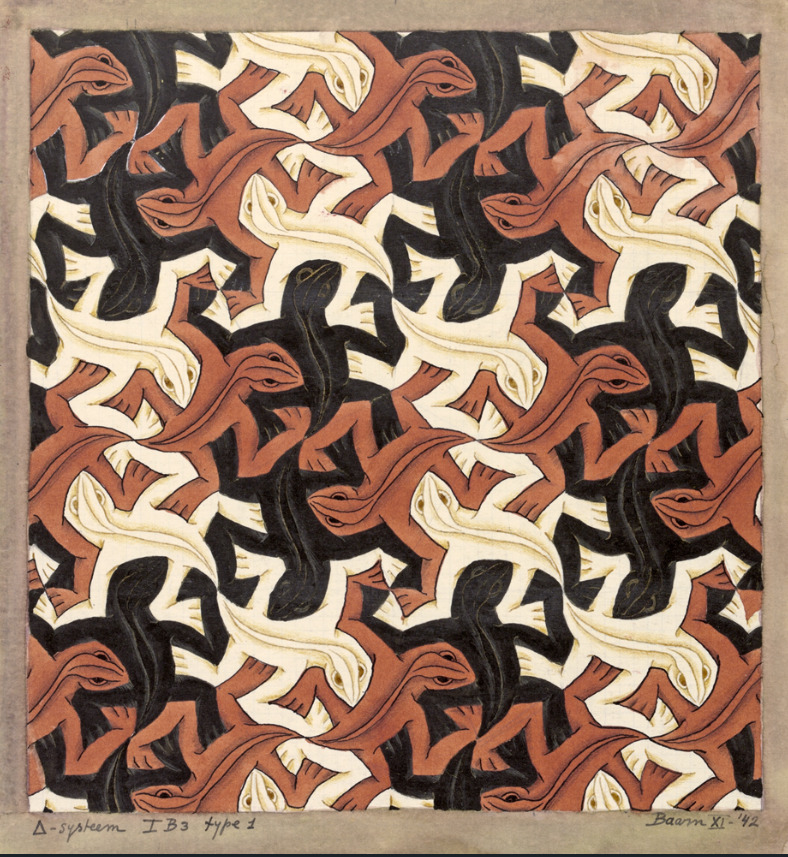
\includegraphics[width=200bp]{lagartos}

\caption{Lizard, M.C. Escher. Fonte: \href{https://www.wikiart.org/en/m-c-escher/lizard-1}{Wikiart}}
\label{lad-fig-1}
\end{figure}

Escher criou esse mosaico transformando um hexágono em um lagarto. Como será que ele fez isso?

Mas, um ladrilhamento nem sempre cobre uma superfície plana. Por exemplo, essa  superfície pode ser a parte externa de uma bola ou de um abajur. Pode ser  a parte interna de um ovo decorado, a pele de uma cobra, um hexágono plano ou uma parede. Assim, neste capítulo, vamos reconhecer, descrever e criar ladrilhamentos, para explorar e percebê-los no ambiente que nos cerca.



\begin{task}{Reconhecendo um ladrilhamento}
\begin{enumerate}
\item Para começarmos, considere as figuras a seguir e decida se elas são ou não um ladrilhamento.

\begin{figure}[H]
\centering
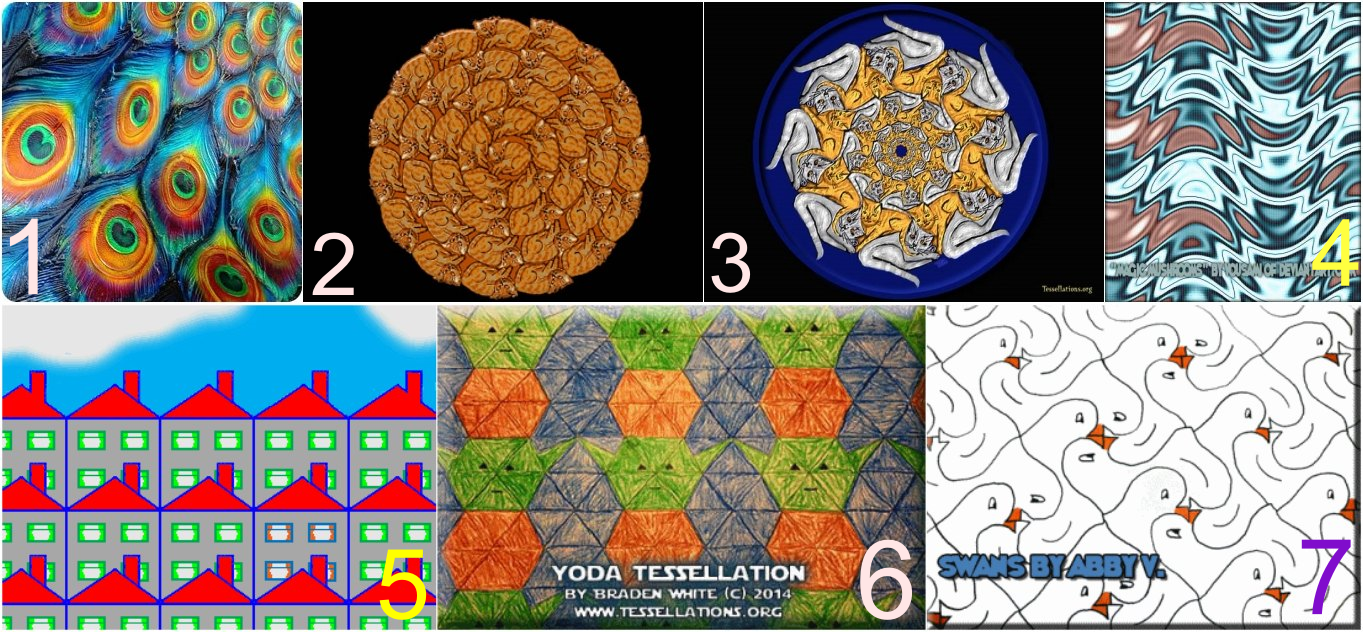
\includegraphics[width=400bp]{ladrilhamento2}
\end{figure}

\item Onde podemos encontrar ladrilhamentos no mundo ao nosso redor? Vamos pensar em alguns exemplos?
\end{enumerate}

\end{task}



\begin{task}{Brincando de ser Escher}
Será que os lagartos podem ser usados para ladrilhar o plano? 

\begin{figure}[H]
\centering
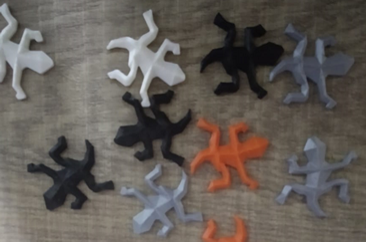
\includegraphics[width=300bp]{ladrilhamento3}

\end{figure}
\end{task}

\arrange{A matemática do ladrilhamento}

Foi possivel fazer um ladrilhamento usando os lagartos? Mas o que os lagartos tem haver com matemática? 

Os ladrilhamentos têm sido amplamente utilizados na arte e na arquitetura desde os tempos antigos, mas o que há por trás disso é a matemática. A teoria é extensa, mas explicaremos alguns princípios básicos para aproximar do que está por trás de belas obras de arte. Quando se trata de ladrilhamento em matemática, também conhecido como mosaico ou pavimentação, é necessário explicar vários termos técnicos com os quais a geometria opera.

Uma região fundamental é uma forma que é repetida para formar um ladrilhamento. Também é chamado de ladrilho. Na atividade anterior, a peça que foi repetida foi o lagarto.

No caso da matemática, geralmente, trabalha-se com polígonos e nesse caso, para construir um ladrilhamento é necessário observar dois aspectos: 

\begin{itemize}
\item Se dois polígonos intersectam-se, então essa interseção é um lado ou um vértice comum;
\item A distribuição dos polígonos  ao redor de cada vértice é sempre a mesma.
\end{itemize}

Agora, com base nessas informações, será possível continuar...


\begin{task}{Outras experiências}

\begin{enumerate}
\item Peças triangulares de formato irregular podem ser usadas para ladrilhar o plano? O que toma um triângulo irregular?
\item Se os ladrilhos triangulares são congruentes., eles podem ser usados para formar um ladrilhamento? Como você pode saber se tiângulos são congruentes ou não? Explique seu raciocínio
\item Copie a forma de um dos triângulos do encarte em um papel de gramatura mais alta. Recorte o triângulo. Crie um desenho, traçando repetidamente. Verifique se a folha de papel está coberta e se não há espaços entre os triângulos.
\item Os polígonos regulares também podem ser usados para criar ladrilhamentos interessantes. Quais características tomam um polígono regular?
\item Copie a forma do hexágono regular do encarte em um papel de gramatura mais alta. Recorte o hexágono. Crie um novo design usando o mesmo processo usado para os triângulos irregulares no exercício anterior.
\item Escreva um breve parágrafo explicando quais informações geométricas você usou para criar seu design no item anterior deste exercício. Por exemplo, você usou translações, rotações ou reflexões para criar seu design? Você usou uma combinação de tranformações? Em caso afirmativo, quais etapas você seguiu para criar seu design?
\end{enumerate}

\end{task}


\begin{task}{Que formas podem ser usadas para ladrilhar o plano?}
\begin{enumerate}

\item Ladrilhamentos são frequentemente feitos de repetições de um padrão (forma fundamental). 

Que padrão pode-se observar nas figuras a seguir?

\begin{figure}[H]
\centering
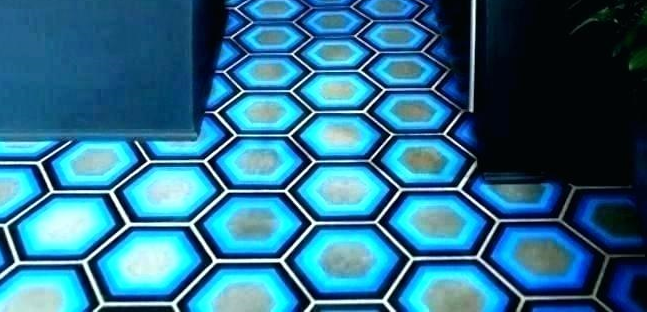
\includegraphics[width=350bp]{ladrilhamento4}
\end{figure}

\begin{figure}[H]
\centering
\begin{minipage}{0.45\textwidth}
\begin{figure}[H]
\centering
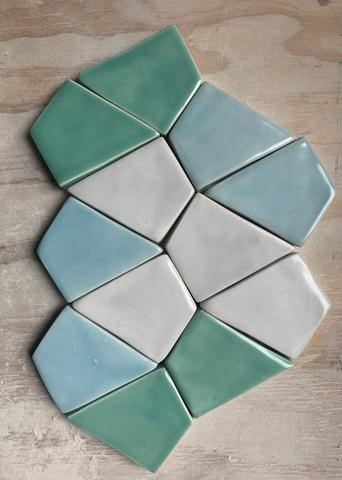
\includegraphics[width=120bp]{ladrilhamento5}

\end{figure}
\end{minipage}
\begin{minipage}{0.45\textwidth}
\begin{figure}[H]
\centering
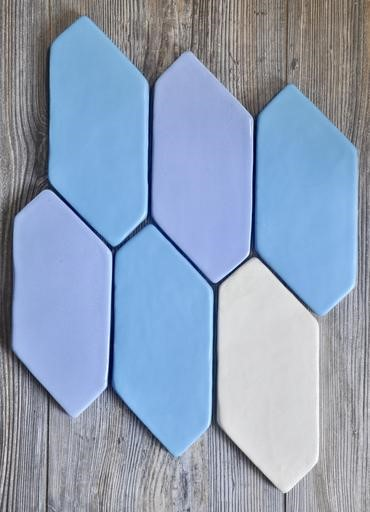
\includegraphics[width=120bp]{ladrilhamento6}

\end{figure}
\end{minipage}
\end{figure}

\begin{table}[H]
\centering
\begin{tabu} to \textwidth{|l|c|c|c|}
\hline
\thead
\makecell{Polígono} & \makecell{Medida de \\ cada ângulo \\ interno} & \makecell{Previsão: \\ O polígono \\ ladrilha o plano?} & \makecell{Resultado: \\ O polígono \\ ladrilha o plano?} \\
\hline
Triângulo Equilátero & & & \\
\hline
Triângulo isóceles & & & \\
\hline
Quadrado & & & \\
\hline
Pentágono regular & & & \\
\hline
Hexágono regular & & & \\
\hline
Octógono regular & & & \\
\hline
Quadrilátero irregular & & & \\
\hline
Pentágono irregular & & & \\
\hline
Hexágono irregular & & & \\
\hline
\end{tabu}
\end{table}

\item Considere um triângulo equilátero. 
	\begin{enumerate}
		\item Esse polígono é regular ou irregular? Registre sua resposta no quadro anterior.
		\item Meça cada ângulo interior e registre suas medidas na tabela.
		\item Você acha que esse polígono ladrilha o plano? Registre sua previsão no quadro.
	\end{enumerate}
\item Usando o triângulo equilátero disponível no encarte, desenhe seu contorno. Mova o triângulo para uma nova posição, para que os doiS triângulos compartilhem um lado comum. Trace o contorno do triângulo novamente. Continue para verificar se o polígono ladrilha o plano. Registre sua conclusão no quadro.
\item Use o mesmo método para descobrir se o triângulo isóceles, quadrado, pentágono regular, hexágono regular e o octógono regular ladrilham o plano. Registre seus resultados no quadro.

\item Desenhe e recorte um quadrilátero irregular
	\begin{enumerate}
		\item Esse polígono ladrilha o plano?
		\item Tente ladrilhar o plano como o quadrilátero. Registre seus resultados no tabela.
		\item Seu quadrilátero é igual ao do seu colega?
	\end{enumerate}
\item Repita as etapas do item b) usando um pentágono irregular e um hexágono irregular desenhado por você.



\item Que polígonos regulares ladrilham o plano? Explique por que alguns polígonos ladrilham o plano mas outras não. Existe um padrão?
\item Explique por que algumas formas irregulares ladrilham o plano mas outras não. Existe um padrão?



\item Com quais dos polígonos a seguir é possível ladrilhar o plano? Explique suas razões.

\begin{figure}[H]
\centering
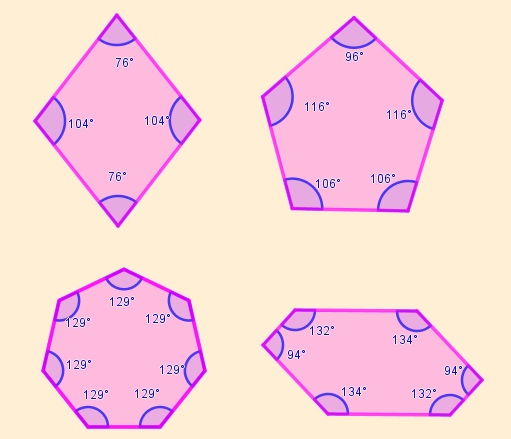
\includegraphics[width=250bp]{ladrilhamento7}
\end{figure}
\end{enumerate}

\end{task}


\explore{O que é um ladrilhamento do plano?}

Um ladrilhamento é um padrão que cobre o plano se sobreposição ou buracos.

\begin{itemize}
\item Somentente três tipos de polígonos regulares ladrilham o plano
\item Alguns tipos de polígonos irregulares ladrilham o plano
\item Polígonos regulares e irregulares ladrilham o plano quando a soma dos vários ângulos que se posicionam e torno de cada vértice é $360^{\circ}$.
\end{itemize}

\begin{figure}[H]
\centering
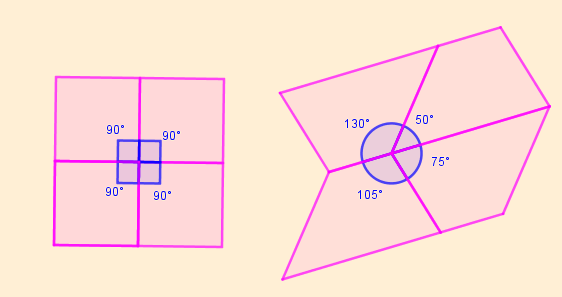
\includegraphics[width=250bp]{ladrilhamento8}
\end{figure}

\begin{task}{Vamos ladrilhar}

\begin{enumerate}
	\item Desenhe três tipos de polígonos regulares que ladrilham o plano. Justifique suas escolhas.
	\item Você consegue identificar dois tipos de polígonos irregulares que podem ser usados para ladrilhar o plano? Utilize o software GeoGebra para justificar a sua escolha.
	\item Alice vai ladrilhar o chão de sua cozinha. Ela poderá escolher cerâmicas com o formato de um octógono regular? Explique.
\end{enumerate}

\end{task}



Em Matemática, dizemos que um conjunto de polígonos é um ladrilhamento \textbf{do plano} (ou \textbf{pavimentação}) se, e somente se, os polígonos do conjunto \textbf{cobrem, sem cruzamentos, um plano}. \textbf{Cobrir}, nessa definição, significa que todo ponto do plano pertence a pelo menos um polígono do conjunto. \textbf{Sem cruzamentos} significa que a interseção de dois polígonos quaisquer tem área nula.

Outras definições importantes são as seguintes:

\begin{itemize}
	\item Os vértices dos polígonos são chamados de \textbf{nós do ladrilhamento}. Observa-se, no entando, que um polígono pode ter mais nós do que vértices. Por exemplo, o polígono $P_2$ na figura a seguir tem oito nós em sua fronteira, mas apenas 5 vértices. Os demais polígonos têm o mesmo número de nós e vértices.

	\begin{figure}[H]
	\centering
	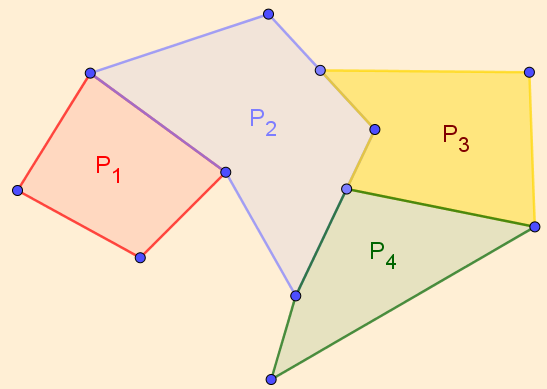
\includegraphics[width=250bp]{ladrilhamento9}
	\end{figure}

	\item Os segmentos de retas que têm por extremos dois nós consecutivos de um mesmo lado do polígono são chamados de \textbf{arestas}.
	\item Um ladrilhamento é lado a lado, se e somente se, toda aresta é lado comum a dois polígonos. Portanto, todo nó na fronteira de um polígono de ladrilhamento é vertice do polígono. Ou seja, ao ladrilhar, um novo polígono é acrescentado se os lados em contato são respectivamente congruentes (figuras A e B), caso contrário o ladrilhamento não é lado a lado (figura C). Neste capítulo o foco será dado aos ladrilhamentos lado a lado.

	\begin{figure}[H]
	\centering
	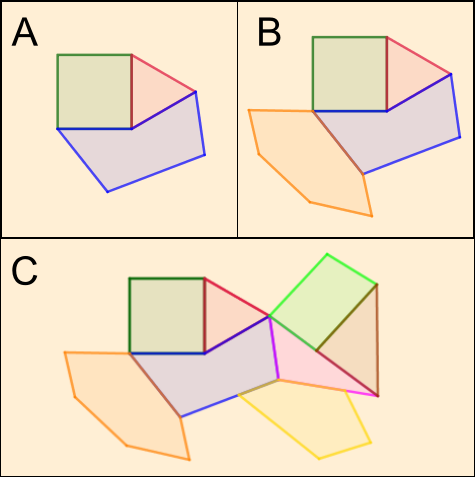
\includegraphics[width=200bp]{ladrilhamento10}
	\end{figure}

	\item Ladrilhamento Monoédricos são aqueles constituídos de polígonos congruentes entre si. Caso os polígonos sejam regulares, os ladrilhamento monoédricos e lado-lado são chamados de \textit{Regulares}.
\end{itemize}

\exercise

\begin{enumerate}
	\item Um ladrilhamento possível usando apenas triângulos equiláteros é o seguinte:

	\begin{figure}[H]
	\centering
	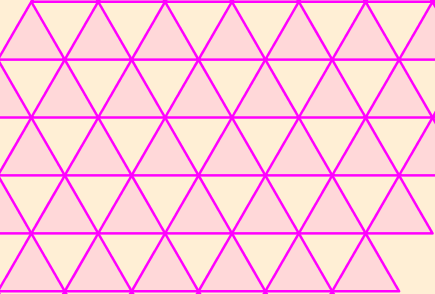
\includegraphics[width=230bp]{ladrilhamento11}
	\end{figure}

	Existem outros? Justifique.

	\item Um pentaminó é uma forma composta por cinco quadrados congruentes conectados pelo menos por um lado.

	\begin{figure}[H]
	\centering
	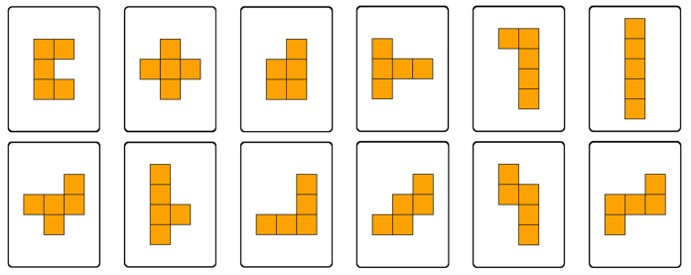
\includegraphics[width=300bp]{ladrilhamento12}

	\caption{Dois jogos de pentaminó. Fonte: \href{https://www.ibilce.unesp.br/departamentos/matematica/eventos/3-cejta/regra-dos-jogos/9-ano---pentamino/}{UNESP.}}
	\end{figure}
	
	\begin{enumerate}
		\item Escolha dois dos pentaminós e tente fazer um ladrilhamento com cada um deles.
		\item Os pentaminós escolhidos ladrilharam o plano?
		\item Explique por que sim ou por que não.
	\end{enumerate}

	\begin{knowledge}
		Um polígono é um $n$-minó se, e somente se, é composto por $n$ quadrados congruentes conectados pelo menos por um lado.

		O termo poliminó foi apresentado pela primeira vez por Solomon Golomb, um matemático do Instituto de Tecnologia da Califórnia, no artigo \textit{Checker Boards and Polyminoes} (publicado no American Mathematical Monthly em dezembro de 1954) e o definiu como "um conjunto de quadrados em ligação simples".
	\end{knowledge}

	\item O diagrama a seguir ilustra um ladrilhamento de quadrados. Adicionando um ponto ao centro de cada quadrado e unindo-os formando quadrados adjacentes, formamos um novo ladrilhamento, que se denomina dual do ladrilhamento original.

	\begin{figure}[H]
	\centering
	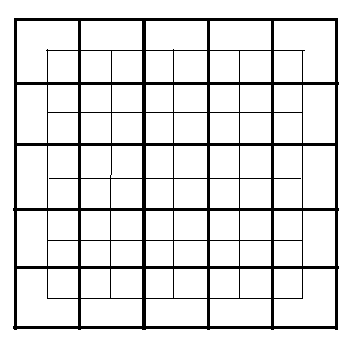
\includegraphics[width=150bp]{ladrilhamento13}
	\end{figure}

	\begin{enumerate}
		\item Que tipo de ladrilhamento é o dual do ladrilhamento de quadrados original?
		\item Desenhe um ladrilhamento de hexágonos regulares. Desenhe e descreva o seu dual;
		\item Desenhe um ladrilhamento de triângulos equiláteros. Desenhe e descreva o seu dual.
	\end{enumerate}
\end{enumerate}


\explore{polígonos de mesmo tipo}

Os ladrilhamentos com peças quadrangulares são comuns nos cômodos de nossas casas. As peças podem ser pintadas, esculpidas ou possuis saliencias e combinadas formam as decorações dos ambientes.

\begin{figure}[H]
\centering
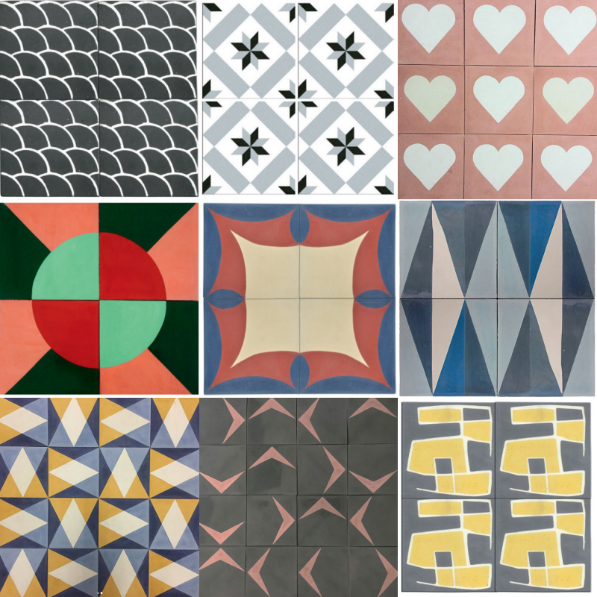
\includegraphics[width=180bp]{ladrilhamento14}
\end{figure}

Também existem ladrilhamento hexagonais, apesar de menos usuais. Eles são encontrados em algumas pavimentações de ruas e áreas externas, nos favos, onde é armazenado o mel das abelhas. Também são comuns na confeção de colchas de retalhos, guardanapos ou colchas de crochê.

\begin{figure}[H]
\centering
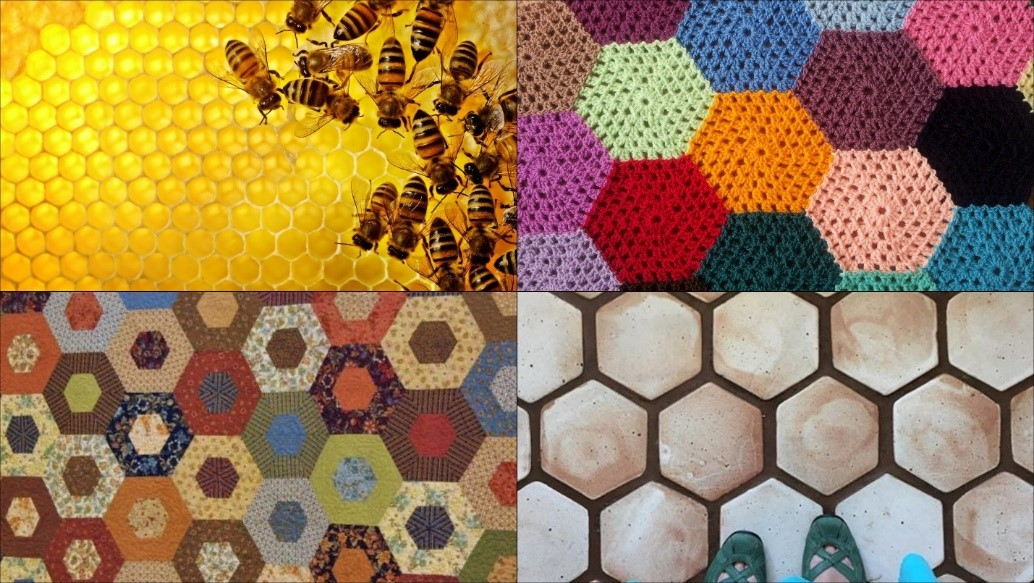
\includegraphics[width=250bp]{ladrilhamento15}
\end{figure}

Uma pergunta que ainda não respondemos nessa seção foi: quais polígonos de mesmo tipo pavimentam o plano? Por que e como isso ocorre?

Um fato conhecido é que a medida dos ângulos internos de um polígono regular de $n$ lados é $\displaystyle \frac{180^{\circ}(n-2)}{n}$. Assim, para que se tena um ladrilhamento formado exclusivamente por polígonos regulares de $n$ lados é preciso que a medida do ângulo interno ($a_n$) seja um divisor de $360^{\circ}$, ou seja,

\begin{equation*}
\frac{180^{\circ}(n-2)}{n}=180^{\circ} \left(1 - \frac{2}{n}\right)=\frac{360^{\circ}}{m},
\end{equation*}
para algum número natural $m\geq1$.

Daí vem

\begin{equation*}
1-\frac{2}{n}=\frac{2}{m}.
\end{equation*}

Logo,
\begin{equation*}
\frac{1}{m}+\frac{1}{m}=2
\end{equation*}

Como $n$ é o número de lados de um polígono regular, é um número natural maior ou igual a três. E como $m$ também é um número natural, as únicas soluções inteiras e positivas, possíveis para a equação anterior são $n=3$ (com $m=6$), $n=4$ (com $m=4$) e $n=6$ (com $m=3$). Essas soluções nos dão exatamente três ladrilhamentos e consistem em distribuir ao redor de cada vértice ou 6 triângulos equiláteros, ou 4 quadrados ou 3 hexágonos regulares.

Assim, podemos concluir que um ladrilhamento é um padrão composto de formas (ladrilhos) que cobrem completamente o plano sem espaços ou sobreposições.



Mas será que podemos usar mais de um tipo de polígono para ladrilhar o plano?


\explore{polígonos de tipos diferentes}



\begin{task}{Ladrilhando o plano com outros polígonos}
\begin{enumerate}
	\item Escolha dois polígonos regulares diferentes que possam ser usados para criar um ladrilhamento.
	\begin{enumerate}
		\item Quais polígonos foram escolhidos?
		\item Você conseguiu realizar o ladrilhamento? Explique.
		\item Desenhe o ladrilhamento usando papel milimetrado usando os dois polígonos.
		\item É possível cobrir um nó do ladrilhamento usando apenas dois polígonos? Justifique.
	\end{enumerate}
\end{enumerate}

\begin{enumerate}
	\item Escolha três polígonos regulares diferentes que possam ser usados para criar um ladrilhamento.
	\begin{enumerate}
		\item Quais polígonos foram escolhidos?
		\item Você conseguiu realizar o ladrilhamento? Explique.
		\item É possível cobrir um nó do ladrilhamento usando apenas dois polígonos? Justifique.
	\end{enumerate}
\end{enumerate}


\end{task}

Mais atividades poderiam ser adicionadas nessa seção


Os ladrilhamentos lado-lado cujas peças são regulares, mas não congruentes entre si, são denominadas de ladrilhamentos semirregulares ou \textit{arquimedianos}. Nessa seção pretende-se investigar quais os tipos de ladrilhamentos lado-lado, cujos ladrilhos são polígonos regulares de mais de um tipo, existem. Alguns desses ladrilhamentos são encontrados em revestimento de pisos. O mais comum é o formado por quadrados, triângulos equiláteros e hexágonos regulares.

\begin{figure}[H]
\centering
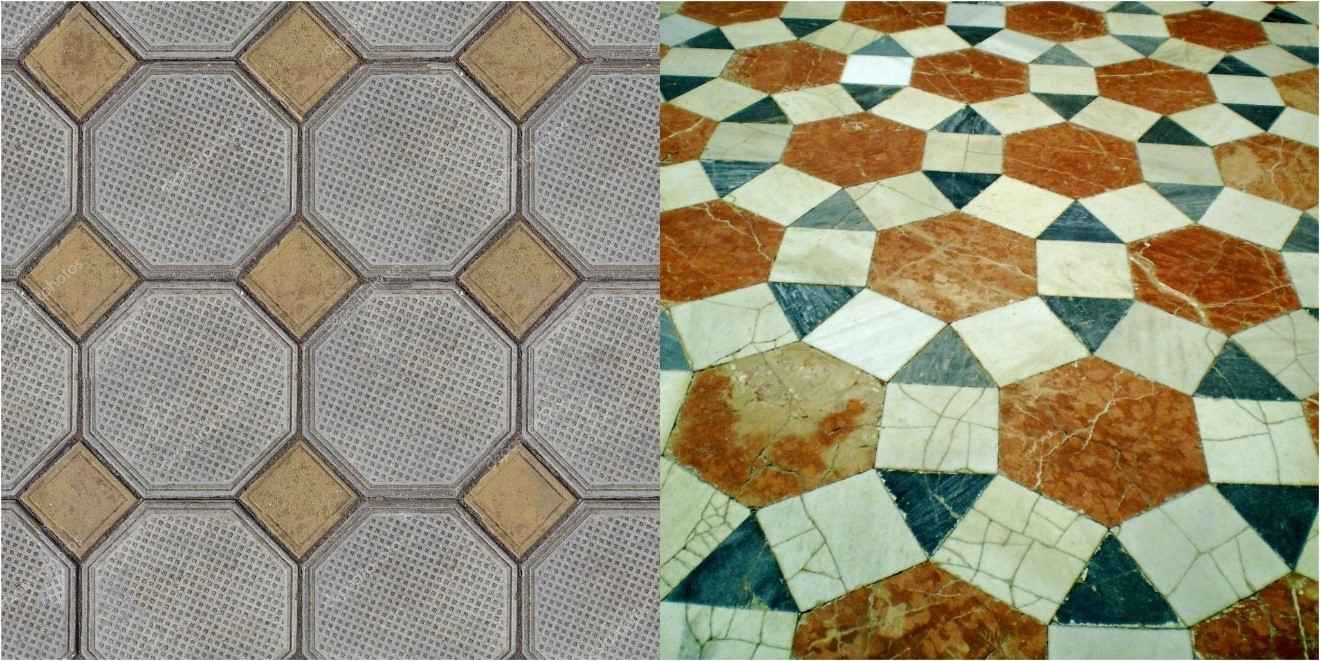
\includegraphics[width=300bp]{ladrilhamento18}
\end{figure}

Um arranjo de polígonos ao redor de um nó é denominado de \textbf{configuração}. E existe uma notação para ela, que se deve ao número de lados dos polígonos que constituemo arranjo. Por exemplo, a configuração (4,8,8) significa que ao redor de um nó há um quadrado, um octágono e um octágono, nesta ordem e em qualquer nó dessa pavimentação.

Já a configuração (3,4,6,4) significa que o redor de um nó há um triângulo, um quadrado, um hexágono e um qudrado, nesta ordem e em qualquer nó dess pavimentação.

\begin{figure}[H]
\centering
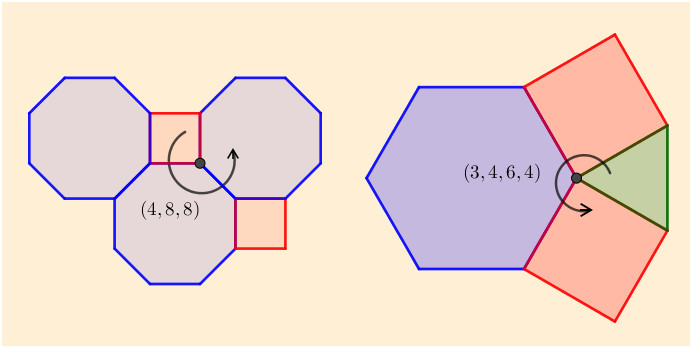
\includegraphics[width=350bp]{ladrilhamento19}
\end{figure}

A existência de ladrilhamentos lado-lado cujas peças são polígonos regulares já era conhecida pelos antigos pitagóricos da Matemática grega. Porém, a primeira pessoa a exibir os ladrilhamentos regulares e semirregulares foi J. Kepler em um trabalho publicado no início do século XVII, onde consta o seguinte resultado:

\begin{description}
\item [Teorema de Kepler] Existem exatamente 11 maneiras de se cobrir o plano utilizando-se exclusivamente polígonos regulares sujeitos às seguintes condições:

\begin{itemize}
	\item Se dois polígonos regulares \textbf{intersectam-se}, então essa interseção é um lado ou um vértice comum.
	\item A distribuição dos polígonos regulares ao redor de cada vértice é sempre a mesma.
\end{itemize}
\end{description}

\begin{knowledge}
Johannes Kepler (1571-1630), em sua obra \textit{Harmonia do Mundo}, de 1619,trouxe as primeiras investigações referentes à teoria da pavimentação do plano eublidiano utilizando polígonos regualres, apontando um tratamento matemático para o problema.
\end{knowledge}

\arrange{pólígonos de tipos diferentes}


Considerando que em torno de um nó podemos colocar um númer $k$ de polígonos regulares, e que $60^{\circ}$ é o menor ângulo interno de um polígono regular, então o maior valor de $k$ é dado por $\displaystyle \frac{360^{\circ}}{60^{\circ}} = 6$, que corresponde a 6 triângulos equiláteros. Por outro lado, o menor número de polígonos necessários para realizar um ladrilhamento em torno de um nó é 3, logo $3\leq k \leq 6$.

Observa-se então que será possível construir ladrilhamentos do plano com 3, 4, 5, ou 6 polígonos regulares em torno de cada nó.

\begin{figure}[H]
\centering
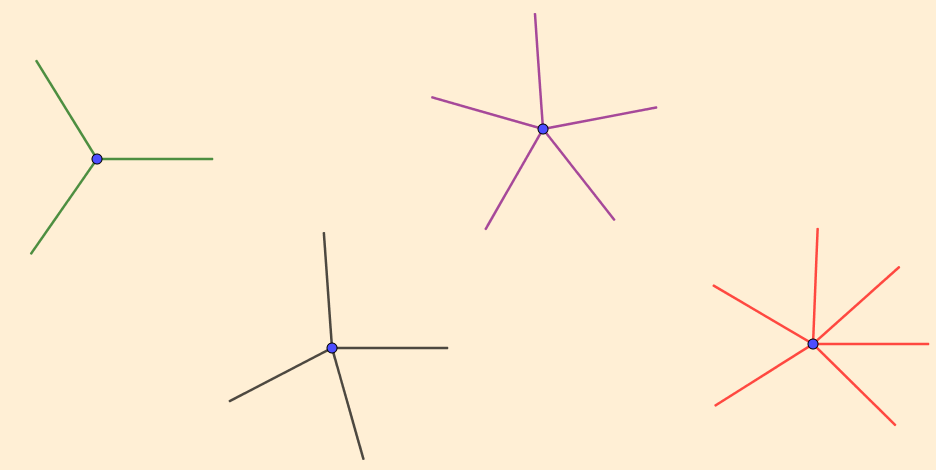
\includegraphics[width=300bp]{ladrilhamento21}

\end{figure}

Examinaremos cada um dos casos separadamento.

Considerando $k=3$, ou seja, supondo que três polígonos regulares são arranjados em torno de um nó de modo que não haja nem lacunas nem superposições, o primeiro com $n_1$ lados, o segundo com $n_2$ lados e o terceiro com $n_3$ lados.

\begin{figure}[H]
\centering
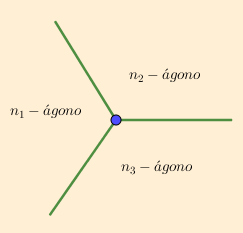
\includegraphics[width=200bp]{ladrilhamento22}

\end{figure}

Como o ângulo interno de cada $n_i$-ágono, com $i=1,2,3$ é dado por

\begin{equation*}
180^{\circ}\left(1-\frac{2}{n_i}\right)
\end{equation*}

E como a soma dos ângulos em torno de um nó é $360^{\circ}$, temos

\begin{equation*}
180^{\circ}\left(1-\frac{2}{n_1}\right)+180^{\circ}\left(1-\frac{2}{n_2}\right)+180^{\circ}\left(1-\frac{2}{n_3}\right)=360^{\circ}.
\end{equation*}

Daí,

\begin{equation*}
\frac{1}{n_1}+\frac{1}{n_2}+\frac{1}{n_3}=\frac{1}{2}
\end{equation*}

Para determinar as soluções inteiras e positivas da equação anterior, vamos supor, sem perda de generalidade, que $n_1\leq n_2\leq n_3$.

Logo,

\begin{equation*}
\frac{1}{n_2}\leq\frac{1}{n_1},\quad \frac{1}{n_3}\leq\frac{1}{n_1},
\end{equation*}

e portanto,

\begin{equation*}
\frac{1}{2}=\frac{1}{n_1}+\frac{1}{n_2}+\frac{1}{n_3}\leq\frac{1}{n_1}+\frac{1}{n_1}+\frac{1}{n_1}=\frac{3}{n_1},
\end{equation*}

ou seja, $n_1\leq6$.

Suponhamos que $n_1=3$, ou seja, que um dos polígonos dispostos ao redor do nó seja um trângulo equilátero. Então,

\begin{equation*}
\frac{1}{3}+\frac{1}{n_2}+\frac{1}{n_3}=\frac{1}{2}.
\end{equation*}

Daí,

\begin{equation*}
\frac{1}{n_2}+\frac{1}{n_3}=\frac{1}{6}.
\end{equation*}

Ou ainda,

\begin{equation*}
\frac{1}{n_3}=\frac{n_2-6}{6n_2},
\end{equation*}

logo, $n_2\geq7$.

Por outro lado, como $n_2\geq n_3$, temos,

\begin{equation*}
\frac{n_2-6}{6n_2}=\frac{1}{n_3}\leq\frac{1}{n_2},
\end{equation*}

O que implica $n_2\leq12$.

Assim, substituindo os valores possíveis para $n_2$ e como $n_3$ é um número inteiro, obtemos as seguintes soluções:

\begin{table}[H]
\centering
\setlength\tabcolsep{5mm}
\begin{tabu} to \textwidth{|c|c|c|}
\hline
\thead
$\bm{n_1}$ & $\bm{n_2}$ & $\bm{n_3}$ \\
\hline
$3$ & $7$ & $42$ \\
\hline
$3$ & $8$ & $24$ \\
\hline
$3$ & $9$ & $18$ \\
\hline
$3$ & $10$ & $15$ \\
\hline
$3$ & $12$ & $12$ \\
\hline
\end{tabu}
\end{table}

Suponhamos agora que $n_1=4$, ou seja, que um dos polígonos dispostos ao redor do nó seja um quadrado. Então,

\begin{equation*}
\frac{1}{4}+\frac{1}{n_2}+\frac{1}{n_3}=\frac{1}{2}.
\end{equation*}

Daí,

\begin{equation*}
\frac{1}{n_2}+\frac{1}{n_3}=\frac{1}{4}.
\end{equation*}

Ou ainda,

\begin{equation*}
\frac{1}{n_3}=\frac{n_2-4}{4n_2},
\end{equation*}

logo, $n_2\geq7$.

Por outro lado, como $n_2\geq n_3$, temos,

\begin{equation*}
\frac{n_2-4}{4n_2}=\frac{1}{n_3}\leq\frac{1}{n_2},
\end{equation*}

o que implica $n_2\leq8$.

Assim, substituindo os valores possíveis para $n_2$ e como $n_3$ é um número inteiro, obetemos as seguintes soluções:

\begin{table}[H]
\centering
\setlength\tabcolsep{5mm}
\begin{tabu} to \textwidth{|c|c|c|}
\hline
\thead
$\bm{n_1}$ & $\bm{n_2}$ & $\bm{n_3}$ \\
\hline
$4$ & $5$ & $20$ \\
\hline
$5$ & $6$ & $12$ \\
\hline
$4$ & $8$ & $8$ \\ 
\hline
\end{tabu}
\end{table}

Procedendo de forma análoga, considerando $n_1 = 5$, temos $5\leq n_2 \leq6$ e uma única solução da equação

\begin{equation*}
\frac{1}{5}+\frac{1}{n_2}+\frac{1}{n_3}=\frac{1}{2}
\end{equation*}

é $n_2=5$ e $n_3=10$. E, considerando $n_1=6$, a única solução é $n_2 = 6$ e $n_3=6$.

Portanto, as soluções inteiras positivas da equação

\begin{equation*}
\frac{1}{n_1}+\frac{1}{n_2}+\frac{1}{n_3}=\frac{1}{2},
\end{equation*} 

estão descritas na tabela a seguir:

\begin{table}[H]
\setlength\tabcolsep{5mm}
\centering
\begin{tabu} to \textwidth{|c|c|c|}
\hline
\thead
$\bm{n_1}$ & $\bm{n_2}$ & $\bm{n_3}$ \\
\hline
$3$ & $7$ & $42$ \\
\hline
$3$ & $8$ & $24$ \\
\hline
$3$ & $9$ & $18$ \\
\hline
$3$ & $10$ & $15$ \\
\hline
$3$ & $12$ & $12$ \\
\hline
$4$ & $5$ & $20$ \\
\hline
$4$ & $6$ & $12$ \\
\hline
$4$ & $8$ & $8$ \\
\hline
$5$ & $5$ & $10$ \\
\hline
$6$ & $6$ & $6$ \\
\hline
\end{tabu}
\end{table}

Considerando $k=4$, ou seja, supondo que quatro polígonos regulares são arranjados em torno de um nó de modo que não haja nem lacunas nem superposições, o primeiro com $n_1$ lados, o segundo com $n_2$ lados, o terceiro com $n_3$ lados e o quarto com $n_4$ lados.

\begin{figure}[H]
\centering
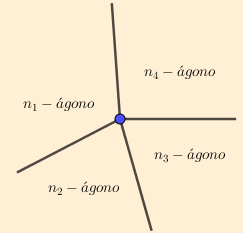
\includegraphics[width=200bp]{ladrilhamento23}
\end{figure}

As possíveis combiunações de quatro polígonos regulares ao redor do nó corresponde a determinar as soluções inteiras e positivas da equação:

\begin{equation*}
180^{\circ}\left(1-\frac{2}{n_1}\right)+180^{\circ}\left(1-\frac{2}{n_2}\right)+180^{\circ}\left(1-\frac{2}{n_3}\right)+180^{\circ}\left(1-\frac{2}{n_4}\right)=360^{\circ},
\end{equation*}

que equivale a

\begin{equation*}
\frac{1}{n_1}+\frac{1}{n_2}+\frac{1}{n_3}+\frac{1}{n_4}=1
\end{equation*}

Repetindo o argumento anterior, é possível verificar que as únicas soluções inteiras e positivas dessa última equação, com $3\leq n_1\leq n_2 \leq n_3 \leq n_4$, são as seguintes

\begin{table}[H]
\centering
\setlength\tabcolsep{5mm}
\begin{tabu} to \textwidth{|c|c|c|c|}
\hline
\thead
$\bm{n_1}$ & $\bm{n_2}$ & $\bm{n_3}$ & $\bm{n_4}$ \\
\hline
$3$ & $3$ & $4$ & $12$ \\
\hline
$3$ & $3$ & $6$ & $6$ \\
\hline
$3$ & $4$ & $4$ & $6$ \\
\hline
$4$ & $4$ & $4$ & $4$ \\
\hline
\end{tabu}
\end{table}

Analogamente ao feito anteriormente, a classificação das possíveis combinações de $k=5$ polígonos regulares em torno de um nó de modo que não haja nem lacunas nem superposiçõs corresponde a determinação das soluções inteiras e positivas da equação

\begin{equation*}
180^{\circ}\left(1-\frac{2}{n_1}\right)+180^{\circ}\left(1-\frac{2}{n_2}\right)+180^{\circ}\left(1-\frac{2}{n_3}\right)+180^{\circ}\left(1-\frac{2}{n_4}\right)+180^{\circ}\left(1-\frac{2}{n_5}\right)=360^{\circ},
\end{equation*}

que equivale a 

\begin{equation*}
\frac{1}{n_1}+\frac{1}{n_2}+\frac{1}{n_3}+\frac{1}{n_4}+\frac{1}{n_5}=\frac{3}{2}.
\end{equation*}

As únicas soluções inteiras e positivas dessa equação, com $3\leq n_2 \leq n_3 \leq n_4 \leq n_5$, estão descritas na tabela

\begin{table}[H]
\centering
\setlength\tabcolsep{5mm}
\begin{tabu} to \textwidth{|c|c|c|c|c|}
\hline
\thead
$\bm{n_1}$ & $\bm{n_2}$ & $\bm{n_3}$ & $\bm{n_4}$ & $\bm{n_5}$ \\
\hline
$3$ & $3$ & $3$ & $3$ & $6$ \\
\hline
$3$ & $3$ & $3$ & $4$ & $4$ \\
\hline
\end{tabu}
\end{table}

Finalmente, considerando $k=6$ polígonos regulares ao redor de um nó nos leva a determinar as soluções inteiras e positivas da equação

\begin{equation*}
\frac{1}{n_1}+\frac{1}{n_2}+\frac{1}{n_3}+\frac{1}{n_4}+\frac{1}{n_5}+\frac{1}{n_6}=2,
\end{equation*}

cuja única solução é $n_1=n_2=n_3=n_4=n_5=n_6=3$

Resumindo, as possíveis combinações de polígonos regulares que ladrilham o plano estão dispostas na tabela:

\setlength\tabcolsep{5mm}
\begin{longtabu} to \textwidth{|c|c|c|c|c|c|c|}
\hline\endfirsthead
\cellcolor{\currentcolor!80}{\textcolor{white}{$\bm{n_1}$}} & \cellcolor{\currentcolor!80}{\textcolor{white}{$\bm{n_2}$}} & \cellcolor{\currentcolor!80}{\textcolor{white}{$\bm{n_3}$}} & \cellcolor{\currentcolor!80}{\textcolor{white}{$\bm{n_4}$}}& \cellcolor{\currentcolor!80}{\textcolor{white}{$\bm{n_5}$}} & \cellcolor{\currentcolor!80}{\textcolor{white}{$\bm{n_6}$}} & \cellcolor{\currentcolor!80}{\textcolor{white}{\textbf{Configuração}}} \\
\hline
$3$ & $7$ & $42$ & & & & $(3,7,42)$ \\
\hline
$3$ & $8$ & $24$ & & & & $(3,8,24)$ \\
\hline
$3$ & $9$ & $18$ & & & & $(3,9,18)$ \\
\hline
$3$ & $10$ & $15$ & & & & $(3,10,15)$ \\
\hline
$3$ & $12$ & $12$ & & & & $(3,12,12)$ \\
\hline
$4$ & $5$ & $20$ & & & & $(4,5,20)$ \\
\hline
$4$ & $6$ & $12$ & & & & $(4,6,12)$ \\
\hline
$4$ & $8$ & $8$ & & & & $(4,8,8)$ \\
\hline
$5$ & $5$ & $10$ & & & & $(5,5,10)$ \\
\hline
$6$ & $6$ & $6$ & & & & $(6,6,6)$ \\
\hline
$3$ & $3$ & $4$ & $12$ & & & $(3,3,4,12)$ \\
\hline
$3$ & $3$ & $6$ & $6$ & & & $(3,3,6,6)$ \\
\hline
$3$ & $4$ & $4$ & $6$ & & & $(3,4,4,6)$ \\
\hline
$4$ & $4$ & $4$ & $4$ & & & $(4,4,4,4)$ \\
\hline
$3$ & $3$ & $3$ & $3$ & $6$ & & $(3,3,3,3,6)$ \\
\hline
$3$ & $3$ & $3$ & $4$ & $4$ & & $(3,3,3,4,4)$ \\
\hline
$3$ & $3$ & $3$ & $3$ & $3$ & $3$ & $(3,3,3,3,3,3)$ \\
\hline
\end{longtabu}

Quais das combinações/configurações que constam na tabela anterior podem ser estendidas de modo a ladrilhar o plano?

\exercise

\begin{enumerate}

\item O revestimento ilustrado na figura a seguir é de um palácio situado em Granada na Espanha. Foram usados ladrilhos de formas diferentes para criar o padrão.

\begin{figure}[H]
\centering
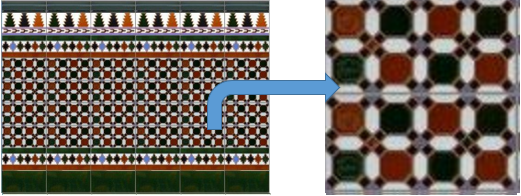
\includegraphics[width=300bp]{ladrilhamento20}

\caption{Fonte: \href{https://alhambratiles.co.uk/collections/granada-range/products/granada-tiles-comares}{Alhambra Tiles}}
\end{figure}

\begin{enumerate}
\item Descreva as formas geométricas que aparecem. Eles são polígonos regulares ou irregulares?
\item Use os encartes para traçar as formas, corte dez peças de cada uma e utilize algumas ou todas para criar pelo menos dois ladrilhamentos distintos (use as quatro formas nos ladrilhamentos construídos).
\item O que foi possível observas nos ladrilhamentos construídos?
\end{enumerate}


	\item Considerando as combinações obtidas para $k=3$
	\begin{table}[H]
	\centering
	\begin{tabu} to \textwidth{|c|c|c|c|}
	\hline
	\thead
	$\bm{n_1}$ & $\bm{n_2}$ & $\bm{n_3}$ & Configuração \\
	\hline
	$3$ & $7$ & $42$ & $(3,7,42)$ \\
	\hline
	$3$ & $8$ & $24$ & $(3,8,24)$ \\
	\hline
	$3$ & $9$ & $18$ & $(3,9,18)$ \\
	\hline
	$3$ & $10$ & $15$ & $(3,10,15)$ \\
	\hline
	$3$ & $12$ & $12$ & $(3,12,12)$ \\
	\hline
	$4$ & $5$ & $20$ & $(4,5,20)$ \\
	\hline
	$4$ & $6$ & $12$ & $(4,6,12)$ \\
	\hline
	$4$ & $8$ & $8$ & $(4,4,8)$ \\
	\hline
	$5$ & $5$ & $10$ & $(5,5,10)$ \\
	\hline
	$6$ & $6$ & $6$ & $(6,6,6)$ \\
	\hline
	\end{tabu}
	\end{table}
	\begin{enumerate}
		\item Com qual delas é possível realizar um ladrilhamento no plano? Justifique.
		\item Justifique porque com algumas dessas combinações não é possível ladrilhar o plano.
	\end{enumerate}

	\item Considerando as combinações obtidas para $k=4$
	\begin{table}[H]
	\centering
	\begin{tabu} to \textwidth{|c|c|c|c|c|}
	\hline
	\thead
	$\bm{n_1}$ & $\bm{n_2}$ & $\bm{n_3}$ & $\bm{n_4}$ & Configuração \\
	\hline
	$3$ & $3$ & $4$ & $12$ & $(3,3,4,12)$ \\
	\hline
	$3$ & $3$ & $6$ & $6$ & $(3,3,6,6)$ \\
	\hline
	$3$ & $4$ & $4$ & $6$ & $(3,4,4,6)$ \\
	\hline
	$4$ & $4$ & $4$ & $4$ & $(4,4,4,4)$ \\
	\hline
	\end{tabu}
	\end{table}

	Observe que ao dispor os polígonos ao redor do nó podemos obter configurações distintas:
	
	\begin{figure}[H]
	\centering
	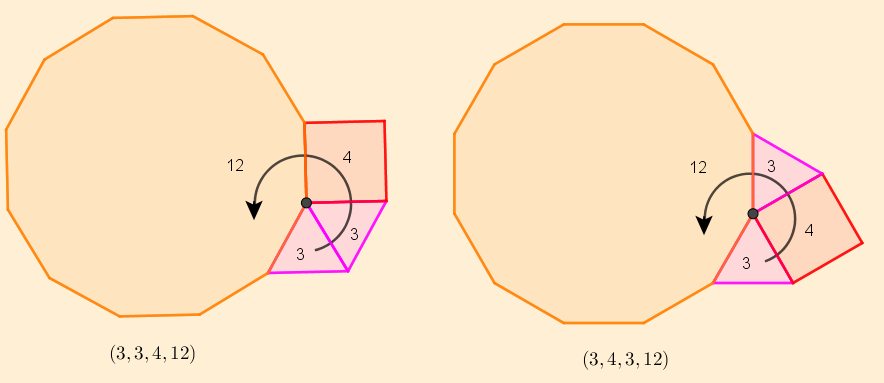
\includegraphics[width=300bp]{ladrilhamento24}

	\end{figure}	
	\begin{figure}[H]
	\centering
	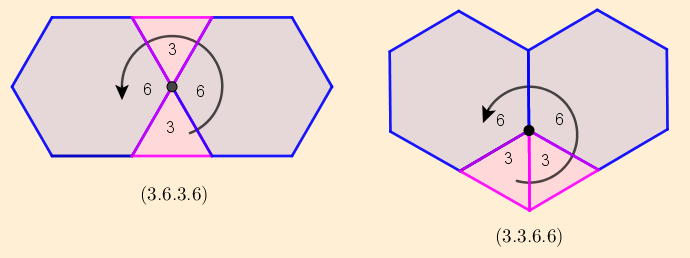
\includegraphics[width=300bp]{ladrilhamento25}

	\end{figure}	
	\begin{figure}[H]
	\centering
	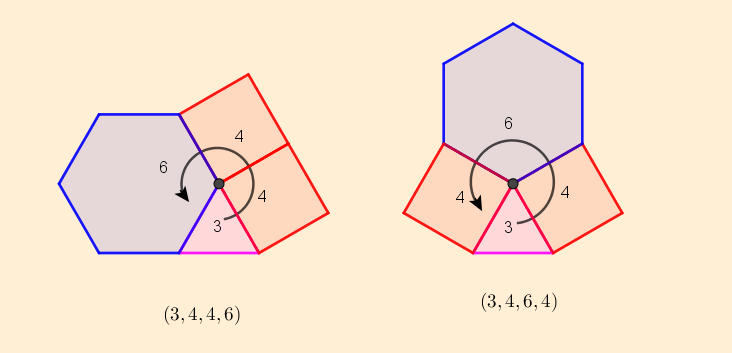
\includegraphics[width=300bp]{ladrilhamento26}

	\end{figure}	

	\begin{enumerate}
		\item Justifique porque elas são diferentes.
		\item Com qual delas é possível ladrilhar o plano?
	\end{enumerate}
	\item \begin{enumerate}
			
		\item Quais combinações foram eliminadas da tabela?

		\begin{tabu} to \textwidth{|c|c|c|c|c|c|c|}
		\hline
		\cellcolor{\currentcolor!80}{\textcolor{white}{$\bm{n_1}$}} & \cellcolor{\currentcolor!80}{\textcolor{white}{$\bm{n_2}$}} & \cellcolor{\currentcolor!80}{\textcolor{white}{$\bm{n_3}$}} & \cellcolor{\currentcolor!80}{\textcolor{white}{$\bm{n_4}$}}& \cellcolor{\currentcolor!80}{\textcolor{white}{$\bm{n_5}$}} & \cellcolor{\currentcolor!80}{\textcolor{white}{$\bm{n_6}$}} & \cellcolor{\currentcolor!80}{\textcolor{white}{\textbf{Configuração}}} \\
		\hline
		$3$ & $7$ & $42$ & & & & $(3,7,42)$ \\
		\hline
		$3$ & $8$ & $24$ & & & & $(3,8,24)$ \\
		\hline
		$3$ & $9$ & $18$ & & & & $(3,9,18)$ \\
		\hline
		$3$ & $10$ & $15$ & & & & $(3,10,15)$ \\
		\hline
		$3$ & $12$ & $12$ & & & & $(3,12,12)$ \\
		\hline
		$4$ & $5$ & $20$ & & & & $(4,5,20)$ \\
		\hline
		$4$ & $6$ & $12$ & & & & $(4,6,12)$ \\
		\hline
		$4$ & $8$ & $8$ & & & & $(4,8,8)$ \\
		\hline
		$5$ & $5$ & $10$ & & & & $(5,5,10)$ \\
		\hline
		$6$ & $6$ & $6$ & & & & $(6,6,6)$ \\
		\hline
		$3$ & $3$ & $4$ & $12$ & & & $(3,3,4,12)$ \\
		\hline
		$3$ & $3$ & $6$ & $6$ & & & $(3,3,6,6)$ \\
		\hline
		$3$ & $4$ & $4$ & $6$ & & & $(3,4,4,6)$ \\
		\hline
		$4$ & $4$ & $4$ & $4$ & & & $(4,4,4,4)$ \\
		\hline
		$3$ & $3$ & $3$ & $3$ & $6$ & & $(3,3,3,3,6)$ \\
		\hline
		$3$ & $3$ & $3$ & $4$ & $4$ & & $(3,3,3,4,4)$ \\
		\hline
		$3$ & $3$ & $3$ & $3$ & $3$ & $3$ & $(3,3,3,3,3,3)$ \\
		\hline
		\end{tabu}

	\item Quais as configurações que fornecem os ladrilhamentos do plano?
\end{enumerate}
\end{enumerate}

Os ladrilhamentos podem ser feitos com dois ou mais polígonos, desde que os ângulos internos onde os vértices dos polígonos se encontram totalizem exatamente $360^{\circ}$.



\explore{translações e reflexões}

Nas seções anteriores construímos ladrilhamentos usando polígonos regulares e irregulares. Mas os ladrilhamentos podem ser construídos combinando esses dois tipos de polígonos e usando uma determinada transformação geométrica



\begin{task}{Como criar um ladrilho usando transformações?}

\begin{enumerate}
	\item Desenhe um hexágono regular em um pedaço de papel, recorte o hexágono e cole-o para uma folha de papelão ou papel o qual deseja construir o ladrilhamento.
	\item Desenhe dois triângulos equiláteros em um pedaço de papel. Verifique se os comprimentos dos lados dos triângulos são iguais as comprimentos dos lados do hexágono. Recorte os triângulos e cole-os na mesma folha de papelão ou papel para que sejam anexados aos lados do hexágono.

	\begin{figure}[H]
	\centering
	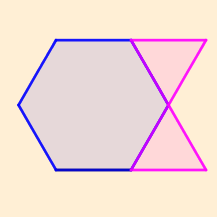
\includegraphics[width=150bp]{ladrilhamento27}

	\end{figure}

	\item Recorte a forma combinada. Trace a forma em uma nova folha de papel. Desloque a forma para que o hexágono se encaixe no espaço formado pelos dois triângulos. Trace ao redor da forma deslocada e repita mais duas vezes.

	\begin{figure}[H]
	\centering
	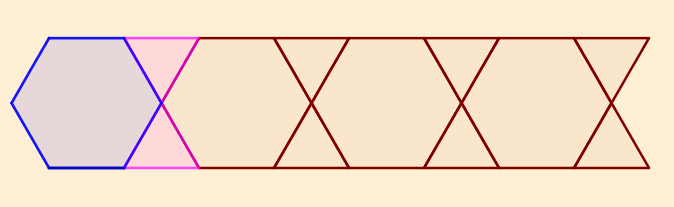
\includegraphics[width=300bp]{ladrilhamento28}

	\end{figure}
	\begin{enumerate}
		\item De que outras maneiras você pode deslocar a forma?
		\item Uma maneira é transladar a peça combinada vertical e horizontalmente para que a base do hexágono esteja agora no topo de um dos triângulos.
	\end{enumerate}
	\item Descreva como usou a transalação para criar os ladrilhamentos. Que outros deslocamentos você poderia usar para obter o mesmo padrão anterior? Explique a diferença.
\end{enumerate}
\end{task}

\begin{task}{identificando as transformações}

\begin{enumerate}
	\item Quais polígonos e quais deslocamentos são usados para criar esse ladrilhamento?
	\begin{figure}[H]
	\centering
	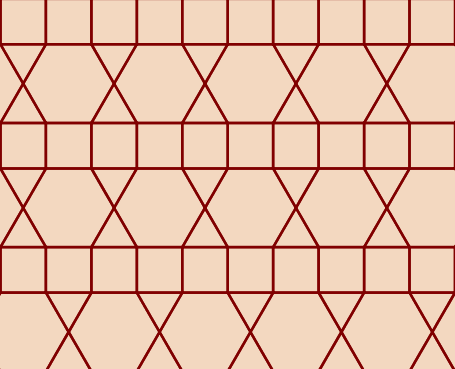
\includegraphics[width=200bp]{ladrilhamento29}

	\end{figure}
	\item Existe a possibildade de ladrilhar o plano usando os mesmos polígonos mas como um padrão diferente?
\end{enumerate}
\end{task}

\exercise

\begin{enumerate}

	\item Anita e Vitória estão tentando descobrir como esse ladrilhamento foi feito.

	\begin{figure}[H]
	\centering
	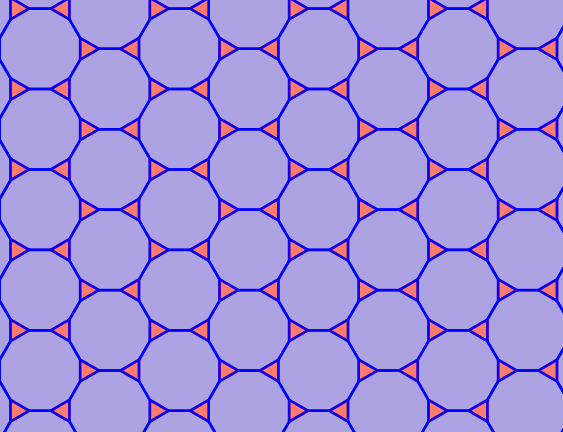
\includegraphics[width=250bp]{ladrilhamento30}

	\end{figure}

	\begin{itemize}
	\item Anita: O ladrilhamento é baseado em refletir os triângulos rosas ao através do dodecágono azul.
	\item Vitória: O ladrilhamento é baseado na translação do dodecágono azul com dois triângulos rosas.
	\end{itemize}

	De quem é a resposta correta? Explique.


	\item 

	\begin{enumerate}
	\item Identifique os dois polígonos regulares que compõe o ladrilhamento.

	\begin{figure}[H]
	\centering
	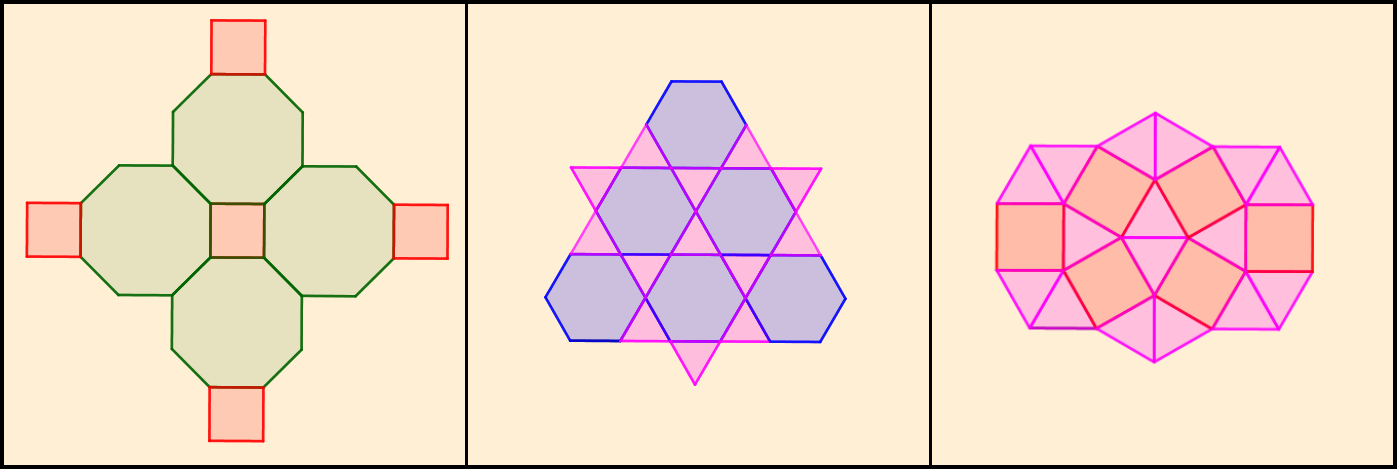
\includegraphics[width=300bp]{ladrilhamento31}

	\end{figure}
		\item Quais tipos de transformações podem ser utilizadas para criar o ladrilhamento?
		\item Qual o padrão observado em cada ladrilhamento?
	\end{enumerate}

	\item A imagem mostra um encaixe formado por figuras irregulares de doze lados. 

	\begin{figure}[H]
	\centering
	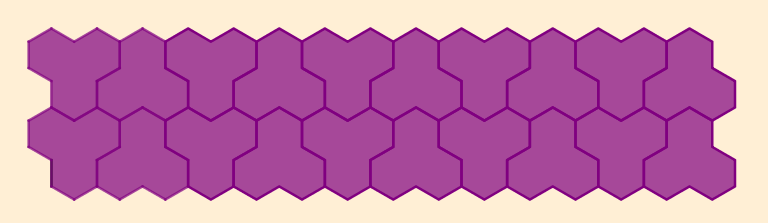
\includegraphics[width=300bp]{ladrilhamento32}

	\end{figure}
	\begin{enumerate}
		\item Explique porque a figura de 12 lados ladrilha o plano perfeitamente.
		\item Usando lápis e papel tente criar uma figura irregular de 10 lados que também cobre um plano.
		\item Explique como foi possível ladrilhar o plano com a figura irregular de 10 lados.
		\item Usando lápis e papel tente criar uma figura irregular de 6 lados que também cobre um plano.
		\item Explique como foi possível ladrilhar o plano com a figura irregular de 6 lados.
	\end{enumerate}

	\item Sabrina está desenhando um papel de parede padronizado por um ladrilhamento. Ela decidiu usar o formato de letra "T" como base. Crie dois ladrilhamentos distindos usando as três letras mostradas a seguir.

	\begin{figure}[H]
	\centering
	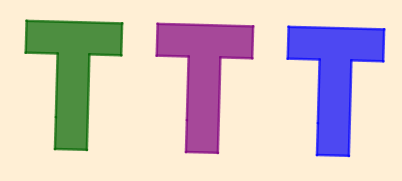
\includegraphics[width=250bp]{ladrilhamento33}

	\end{figure}

	\item Priscila está projetando um azulejo de cozinha que usa dois polígonos regulares diferentes. Ela então usa dois deslocamentos diferentes para criar um ladrilhamento. Use papel quadriculado para projetar um bloco que Priscila poderia usar. Mostre como ladrilhar o plano.

	\item Alice quer fazer uma colcha usando os dois polígonos mostrados.

	\begin{figure}[H]
	\centering
	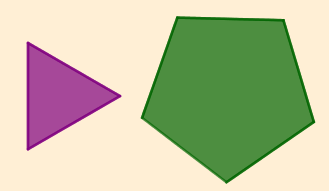
\includegraphics[width=200bp]{ladrilhamento34}

	\end{figure}

	\begin{enumerate}
		\item Ela será capaz de criar um padrão de pavimentação usando essas formas? Explique
		\item Será que Alice consegue fazer um padrão usando pentágonos regulares e triângulos, não necessariamente regulares?
	\end{enumerate}
\end{enumerate}



\arrange{translações e reflexões}

Uma exposição de arte em São Paulo está disponível ao público diariamente de segunda a domingo, praticamente durate 24 horas. Vale a pena reparar nas estações do metrô dessa cidade, quase um verdadeiro museu público e suberrâneo. Mas o que essa exposição tem a ver com matemática?

Em particular, uma das obras denominada momento atropofágico com Oswald de Andrade instalada na estação República do metrô de São Paulo em 1990, chama a atenção

\begin{figure}[H]
\centering
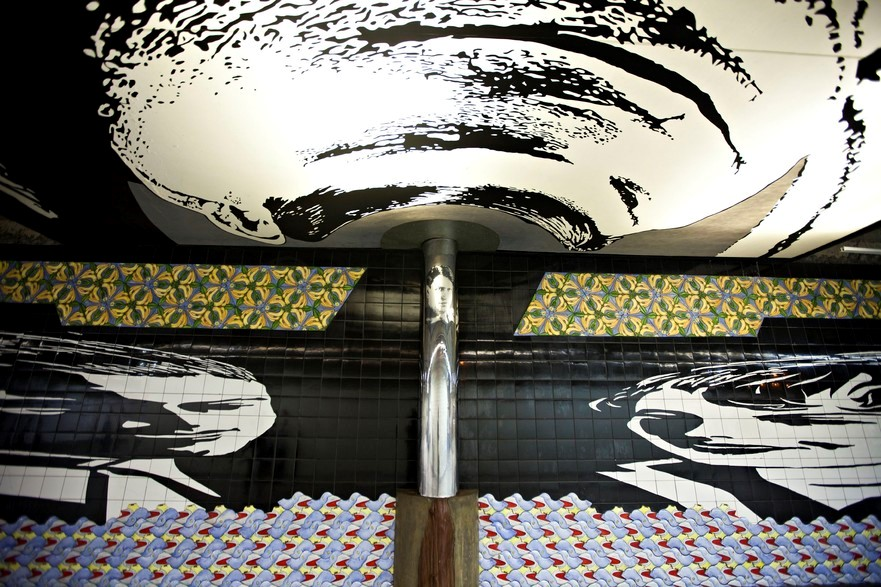
\includegraphics[width=280bp]{ladrilhamento35}

\end{figure}

Você reconhece algum tipo de ladrilhamento nessa obra?

\begin{figure}[H]
\centering
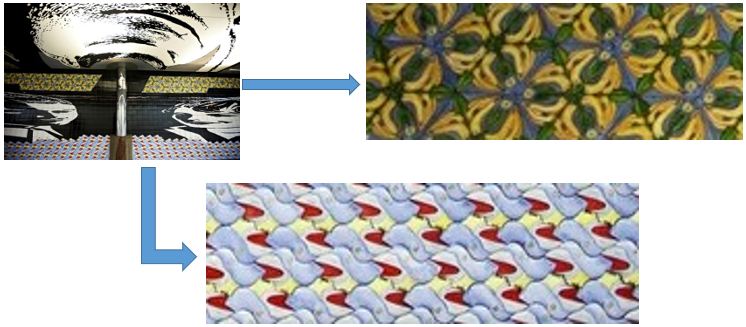
\includegraphics[width=400bp]{ladrilhamento36}

\end{figure}

Você consegue perceber como a transformação geométrica rotação é utilizada para determinar um padrão nesse ladrilhamentos?

\begin{task}{como criar um ladrilho usando rotação}

\begin{enumerate}
	\item Desenhe um triângulo equilátero em um pedaço de papel. Recorte o triângulo e cole-o em uma folha de papelão ou papel para contrução e criar um bloco.
	\item Contorne o seu ladrilho em um pedaço de papel.
	\item Gire o ladrilho $60^{\circ}$ em torno de um vértice até que a lateral do ladrilho caia ao longo da borda do traçado anterior, como ilustra a figura. Trace em torno do lado a lado novamente

	\begin{figure}[H]
	\centering
	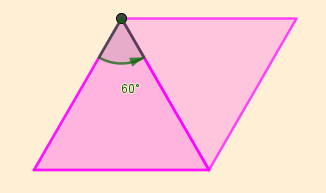
\includegraphics[width=200bp]{ladrilhamento37}

	\end{figure}

	\item Repita o terceiro passo até que uma volta completa tenha sido feita.
	\begin{enumerate}
		\item Que forma você criou?
		\item Quantas vezes você teve que firar o ladrilho para criar essa forma?
	\end{enumerate}

	\item Adicione cores e desenhos ao ladrilhamento para criar uma obra de arte.

	\item Como você pode continuar usando rotações para aumentar o ladrilhamento.

\end{enumerate}


\begin{enumerate}
	\item Descreva como usar a rotação de polígonos para criar um ladrilhamento
	\item Quais tipos de polígonos podem ser usados para fazer um ladrilhamneto com rotações?

	\item Quais polígonos e transformações foram usados para criar essa figura? Justifique.

	\begin{figure}[H]
	\centering
	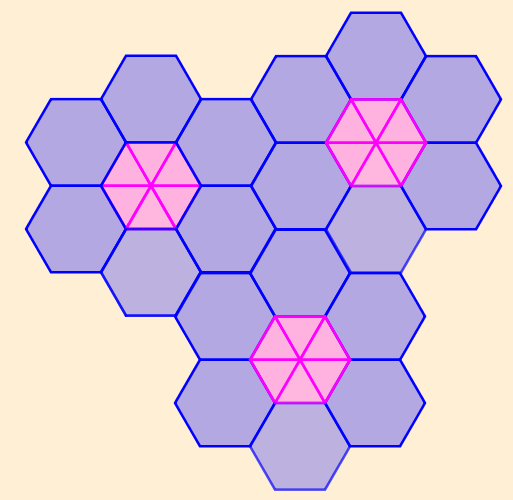
\includegraphics[width=150bp]{ladrilhamento38}

	\end{figure}




\end{enumerate}

\end{task}

\exercise
\begin{enumerate}
	\item
	\begin{enumerate}
	\item Identifique os polígonos usados para criar os seguintes ladrilhamentos:
	\begin{figure}[H]
	\centering
	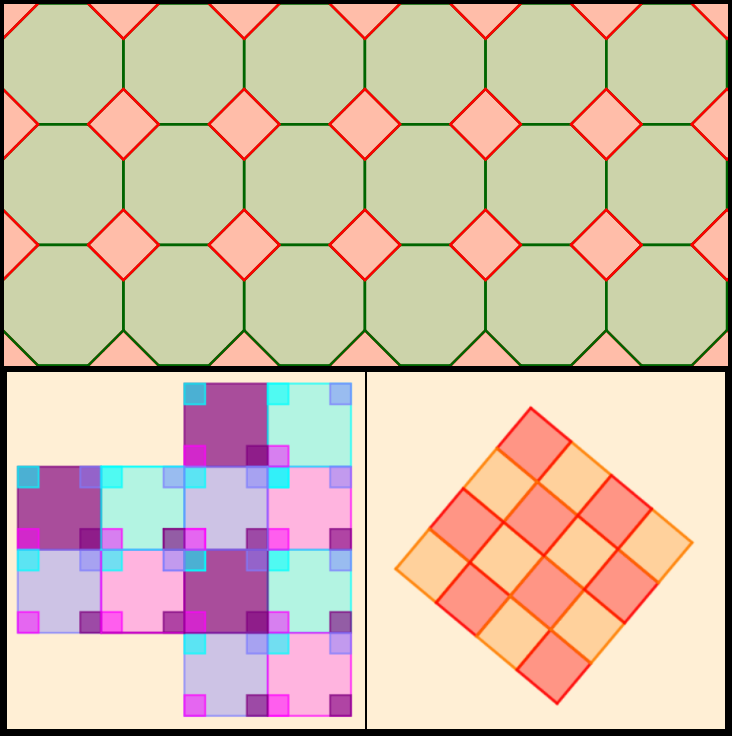
\includegraphics[width=250bp]{ladrilhamento39}

	\end{figure}

	\item Quais as transformações foram usadas?

	\end{enumerate}

	\item A \textbf{Catedral de Notre-Dame de Paris} (em português: "Catedral de Nossa Senhora de Paris") é uma das mais antigas catedrais francesas e foi decorada com vitrais coloridos, como o da imagem:

	\begin{figure}[H]
	\centering
	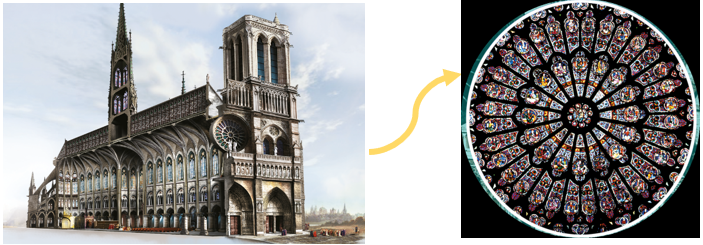
\includegraphics[width=400bp]{ladrilhamento40}
	\end{figure}
	
	\begin{enumerate}
		\item Descreva as tranformações usadas para fazer este vitral
		\item Se você estivesse usando esse padrão para ladrilhar o plano, quais modificações você teria que fazer?

	\end{enumerate}

	\item Crie seu próprio vitral em papel quadriculado. Descreva as etapas que você seguiu para criar o padrão.

	\item Crie um Mosaico usando dois polígonos regulares diferentes e rotações.

	\item Quais das seguintes formas ladrilham o plano?

	\begin{figure}[H]
	\centering
	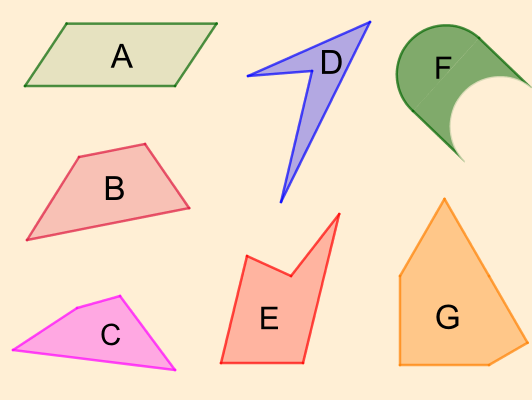
\includegraphics[width=300bp]{ladrilhamento41}

	\end{figure}
	Explique como você decide se uma forma produz ou não um ladrilhamento.

\end{enumerate}

\arrange{Ladrilhamento usando transformações}

Ao observar um ladrilhamento, podemos notar que o ladrilho original, se repete em um padrão. Uma ideia matemática que pode ser enfatizada por meio dos ladrilhos é a simetria. No entanto, uma simetria pode ser encontrada quando duas metades de uma determinada figura são congruentes. Não deve ser confundida com o tipo de simetria que pode ser encontrada em um ladrilhamento. Em termos de um plano infinito, essas simetrias são chamadas de simetrias do plano ou transformações geométricas. Existem simetrias em um plano que movem o ladrilho "padrão" de uma maneira que ainda corresponde exatamente ao original: a translação e a rotação.


\explore{Pavimentação no estilo Escher}

\begin{task}{Como fazer pavimentações no estilo Escher?}
\begin{enumerate}
	\item Desenhe um triângulo equilátero em um papel em brando. Recorte o triângulo e cole-o em uma folha de papel para construção. Recorte o triângulo novamente.

	\item Dentro de cada triângulo, desenhe uma curva que conecta dois vértices adjacentes. Corte ao longo da curva para remover uma peça do triângulo.

	\begin{figure}[H]
	\centering
	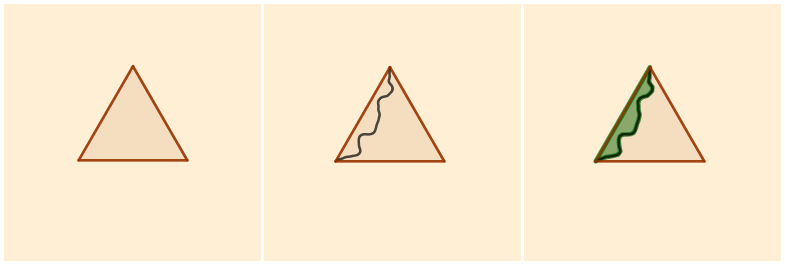
\includegraphics[width=350bp]{ladrilhamento42}

	\end{figure}

	\item Gire a peça que você removeu $60^{\circ}$ no sentido anti-horário sobre o vértice da extremidade superior da curva. Mova a peça para o outro lado do triângulo. Cole a peça no lugar para completar seu ladrilho.

	\begin{figure}[H]
	\centering
	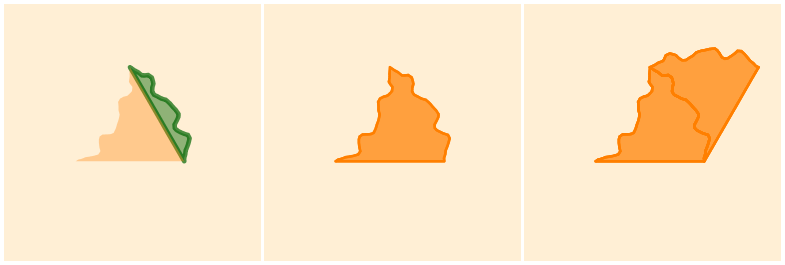
\includegraphics[width=350bp]{ladrilhamento43}

	\end{figure}

	\item Para ladrilhar o plano, trace ao redor do ladrilho. Em seguida, gire e desenhe o ladrilho repetidamente até que se tenha o design pretendido.
	\item Adicione cores e desenhos ao ladrilho para que pareça uma obra de arte.

	\begin{figure}[H]
	\centering
	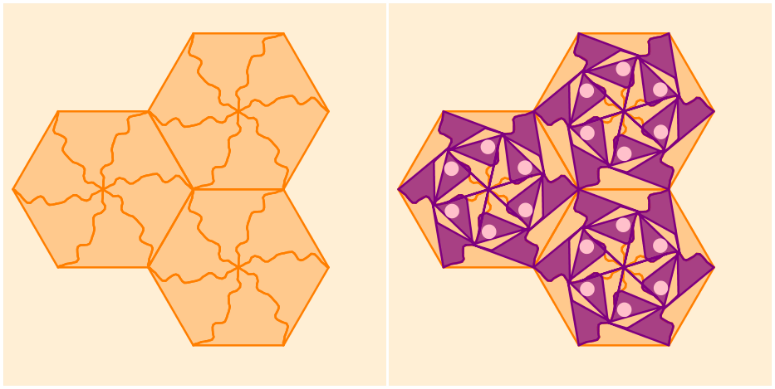
\includegraphics[width=200bp]{ladrilhamento44}

	\end{figure}

	\item Repita as etapas de 1 a 5 usando em paralelogramo e translações para criar outro desenho no estilo Escher.

	\item Você pode usar as transformações para criar ladrilhamentos no estilo Escher, assim como você fez, com polígono regulares e irregulares.
	\begin{enumerate}
		\item Descreva como usar as rotações para criar mosaicos no estilo Escher.
		\item O que você nota sobre a soma das medidas de ângulo nos vértices onde os ladrilhos se encontra?
	\end{enumerate}
\end{enumerate}
\end{task}

\begin{task}{Praticando}

	\begin{enumerate}
		\item Quais transformações foram utilizadas para criar os seguintes ladrilhamentos? Explique sua resposta.

	\begin{figure}[H]
	\centering
	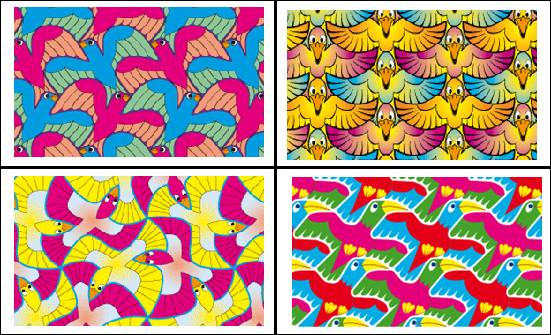
\includegraphics[width=350bp]{ladrilhamento45}

	\end{figure}
		\item Identifique a figura plana que originou cada um dos ladrilhamentos do exercício anterior.

		\item Crie um ladrilhamento no estilo Escher usando um triângulo escaleno a partir de translações.

		\item Crie um ladrilhamento no estilo Escher usando um triândulo equilátero com rotações.

		\item Crie um ladrilhamento no estilo Escher usando quadrados com rotações e translações
	\end{enumerate}


\end{task}


\explore{Polígonos irregulares de mesmo tipo}



Outros polígonos, como triângulos, quadriláteros e hexágonos não regulares também ladrilham o plano.

Na primeira seção desse capítulo, vimos que qualquer triângulo e qualquer quadrlátero ladrilham o plano. Nas atividades a seguir, vamos explorar um pouco mais sobre os ladrilhamentos usando quadriláteros, pentágonos e hexágonos.



\begin{task}{Ladrilhamentos usando quadriláteros}
\begin{enumerate}
	\item Lembre que um paralelogramo é um quadrilátero que possui lados opostos paralelos, com isso, são válidas algumas propriedade, entre elas:
	\begin{itemize}
		\item Os lados opostos são congruentes.
		\item Os ângulos opostos são congruentes.
		\item Os ângulos são dois a dois suplementares
	\end{itemize}
	\begin{figure}[H]
	\centering
	\includegraphics[width=150bp]{ladrilhamento46}

	\end{figure}

	Com base no explicidade acima, será que os paralelogramos podem ladrilhar o plano? Justifique sua resposta.

	\item Um losango (que também é um paralelogramo) fornece um padrão que aparente cubos em perspectiva.

	\begin{figure}[H]
	\centering
	\includegraphics[width=150bp]{ladrilhamento47}

	\end{figure}
	\begin{enumerate}
			\item O que esse losango possui de especial?
			\item Será que é possível construir outro padrão com esses losangos? (Use o GeoGebra ou os losangos do encarte)
	\end{enumerate}

	\item Será que é possível ladrilhar o plano usando trapézios? Justifique.


\item Um trapézio muito interessante, chamado 60-120, quando se trata de ladrilhamento, é o constituído por três triângulos equiláteros.

\begin{figure}[H]
\centering
\includegraphics[width=300bp]{ladrilhamento48}

\end{figure}

\begin{enumerate}
	\item A figura abaixo ilustra um padrão parcial feito com esse trapézio, em um hexágono regular (e como o hexágono pavimenta o plano, basta repetir o padrão hexagonal). Construa outro padrão no hexágono usando apenas trapézios 60-120.

	\begin{figure}[H]
	\centering
	\includegraphics[width=250bp]{ladrilhamento49}

	\end{figure}

	\item Com o trapézio 60-120 também é possível construir padrões do tipo "faixas decorativas". Faça um padrão diferente do apresentado usando trapézios 60-120.

	\begin{figure}[H]
	\centering
	\includegraphics[width=300bp]{ladrilhamento50}

	\end{figure}
\end{enumerate}


\item Use o GeoGebra para verificar se qualquer quadrilátero pode ladrilhar o plano.
\begin{enumerate}
	\item Construa um quadrilátero qualquer no software.
	\item Utilize as transformações geométricas (translações e rotações) para construir o ladrilhamento.
	\item O quadrlátero construído é convexo?
	\item Se não for convexo, ele ainda vai ladrilhar o plano?
\end{enumerate}

\item Os pisos de algumas casa são cobertos por ladrilhos retangulares. O padrão a seguir é denominado espinha de peixe. 

	\begin{figure}[H]
	\centering
	\includegraphics[width=250bp]{ladrilhamento16}

	\caption{Fonte: \href{http://www.tilehomeguide.com/tile-patterns-the-ultimate-quick-read-beginners-guide-including-secrets-of-tile-professionals-revealed/}{The Tile Home Guide}}
	\end{figure}

 Em papel quadriculado, crie dois designs diferentes a partir de ladrilhos retangulares congruentes.
\end{enumerate}

\end{task}

\begin{task}{Ladrilhamento usando pentágonos}

\begin{enumerate}

	\item Um pentágono pode ladrilhar o plano?

Ladrilhamentos feitos com pentágonos não aparecem apenas nas calçadas do Cairo. A figura abaixo ilustra o piso do banheiro de Robert John Jenkis Junior (Bob Jenkis) que fez um arranjo com azulejos pentagonais irregulares para cobrir o pido do banheiro após uma reforma (A história completa sobre essa reforma está no site \href{http://burtleburtle.net/bob/other/bathroom.html}{BurtleBurtle})

\begin{figure}[H]
	\centering
	\includegraphics[width=300bp]{ladrilhamento53.jpg}

\end{figure}

Em 2015 houve uma descoberta no campo da geometria. Essa descoberta foi do 15$^{\circ}$ tipo de pentágono que pode ladrilhar o plano. Quinze tipos diferentes de pentágono podem formar mosaicos, mas o pentágono regular não pode. Por que isso acontece?

\item Algumas calçadas possuem uma pavimentação diferente, denominada "Cairo Tilling"Ou Pavimentação do Cairo. Embora esse seja um padrão matemático, seu nome foi criado devido ao fato de várias ruas do Cairo (no Egito) serem pavimentadas com pedras desse tipo.

	\begin{figure}[H]
	\centering
	\includegraphics[width=250bp]{ladrilhamento17}
	\end{figure}

Observamos que os ladrilhos são pentágonos irregulares.

	\begin{enumerate}
		\item Desenhe um ladrilho pentagonal diferente do apresentado na figura, que possa pavimentar o plano. Explique como ele ladrilhará o plano.
		\item Esse é o único ladrilho pentagonal possível? Compare com seus colegas.
	\end{enumerate}

\end{enumerate}
\end{task}

\begin{task}{A pipa e a flecha}

Parte da rua central de Helsinque na Finlândia foi transformada em uma rua para pedestres e pavimentada com ladrilhos do tipo Penrose. Esses ladrilhos foram inventados pelo matemático inglês Roger Penrose na década de 1970.

\begin{figure}[H]
	\centering
	\includegraphics[width=300bp]{ladrilhamento51}

\end{figure}

Observe que os ladrilhos têm em duas formas diferentes, a pipa e a flecha. Esses quadrláteros podem ser construídos a partir de um pentágono regular.

	\begin{figure}[H]
	\centering
	\includegraphics[width=300bp]{ladrilhamento52}

	\end{figure}
	\begin{enumerate}
		\item Construa pipas e flechas usando um pentágono regular.
		\item Copie as formas em um papel de gramatura mais alta. Recorte-as e crie dois ladrilhamentos diferentes.
		\item Escreva um breve parágrafo explicando quais transformações geométricas você usou para criar seu design no item anterior deste exercício. Por exemplo, você usou translações, rotações ou reflexões para criar seu design? Você usou uma combinação de transformações? Em caso afirmativo, quais etapas você seguiu para criar seu design?
		\item O que esses ladrilhamentos possuem de diferente dos ladrilhamentos utilizando polígonos construídos anteriormente?
	\end{enumerate}
\end{task}

	\begin{knowledge}
	Se os ladrilhos estiverem dispostos de modo a produzir um padrão de repetição regular, o mosaico será deonominado de periódico. Ladrilhamentos periódicos repetem o ladrilho em duas direções e formam padrões em simetria.

	Porém, se o arranjo de ladrilhos produzir um padrão irregular ou aleatório, o mosaico será denominado aperiódico. Esses ladrilhamentos não têm simetria de translação e o padrão não pode ser repedito periodicamenteo apenas cobrindo uma parte do plano. Alguns dos exemplos mais conhecidos de padrões de ladrilhamento aperiódicos são os ladrilhos de Penrose.
	\end{knowledge}


\begin{task}{Padrões com pentágonos irregulares}

\begin{enumerate}

\item Uma forma de determinar padrões com pentágonos irregulares é considerar os duais de padrões com polígonos regulares de tipos diferentes com a mesma configuração em todo o nó, especialmente os que possuem cinco polígonos ao redor do nó.

Ao considerar o padrão (3,3,3,3,6), encontramos um padrão com pentágonos irregulares.

\begin{figure}[H]
	\centering
	\includegraphics[width=200bp]{ladrilhamento54}

\end{figure}

Será possível encontrar esse tipo de padrão em outros ladrilhamentos com os polígonos regulares de tipos diferentes que possuem 5 polígonos ao redor do nó?

	Experimente o padrão (3,3,4,3,4).

	\begin{figure}[H]
	\centering
	\includegraphics[width=200bp]{ladrilhamento55}

	\end{figure}

\item 	E sem usar o padrão dual, será que é possível determinar um padrão com pentágonos partindo do ladrilhamento composto por quadrados?

	\begin{figure}[H]
	\centering
	\includegraphics[width=250bp]{ladrilhamento56}

	\end{figure}
\end{enumerate}
\end{task}

\begin{task}{Ladrilhamento usando hexágonos}
A parede de um banheiro foi coberta por ladrilhos hexagonais não regulares:

	\begin{figure}[H]
	\centering
	\includegraphics[width=350bp]{ladrilhamento57}

	\end{figure}
	\begin{enumerate}
		\item Qual a condição necessária para que um hexágono qualquer ladrilhe o plano?
		\item Construa um hexágono irregular com lados opostos paralelos congruentes.
		\item Esse hexágono ladrilha o plano? Justifique sua resposta.
		\item O hexágono que você construiu é convexo? E se não for convexo, a resposta dada ao item b) continua válida?
		\item Qual transformação foi utilizada para construir o ladrilhamento?
	\end{enumerate}
\end{task}


\arrange{Polígonos irregulares de mesmo tipo}
Nessa seção podemos concluir que se o polígono é qualquer e possui três ou quatro lados, convexo ou não, então ele pavimenta o plano. Se o polígono possui cinco ou seis lados, então pavimenta o plano em casos especiais.

\newpage

